\documentclass[12pt,a4paper,oneside]{article}
\usepackage[a4paper,left=2cm,right=1cm,top=2cm,bottom=2cm]{geometry}

\usepackage{polyglossia}
\setmainlanguage{russian}
\PolyglossiaSetup{russian}{indentfirst=true}

\usepackage{fontspec}
\defaultfontfeatures{Mapping=tex-text}

\setmainfont{Times New Roman}
\setromanfont{Times New Roman}
\setsansfont{Arial}
\setmonofont{Courier New}

\newfontfamily{\cyrillicfont}{Times New Roman}
\newfontfamily{\cyrillicfontrm}{Times New Roman}
\newfontfamily{\cyrillicfonttt}{Courier New}
\newfontfamily{\cyrillicfontsf}{Arial}

\usepackage{graphicx}
\graphicspath{{pics/}}

\usepackage{float}
\floatstyle{plaintop}
\restylefloat{table}

\usepackage{color, listings}
\lstset{
  basicstyle=\footnotesize\ttfamily,
  inputpath=src/,
  numbers=left,
  showstringspaces=false,
  %upquote=true,
  xleftmargin=\parindent,
}



% 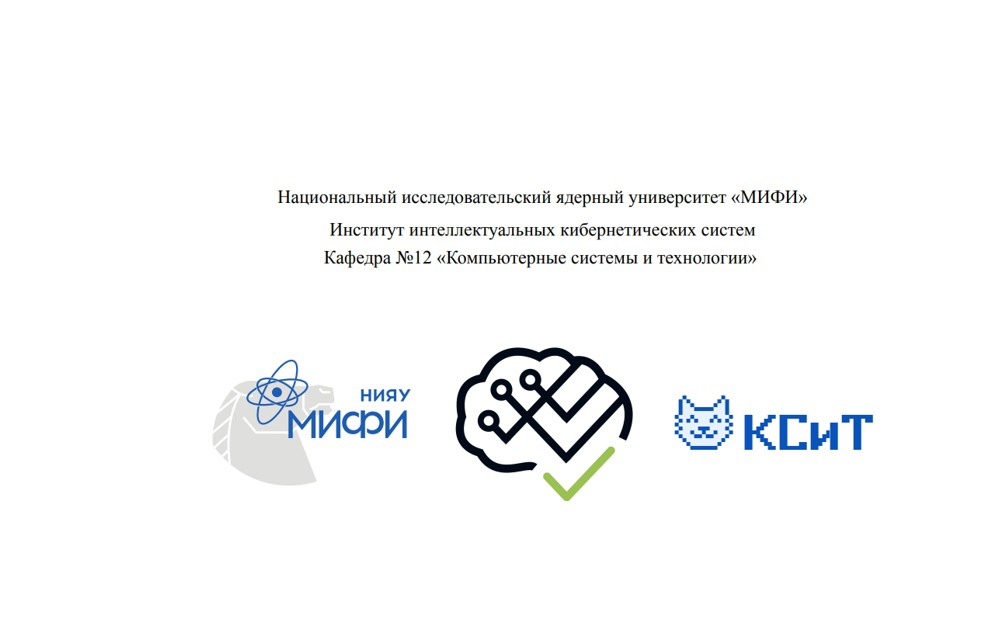
\includegraphics[width=10.975cm]{pics/title.jpg}

% \maketitle

  

\begin{document}

\begin{titlepage}
    \begin{center}
      \begin{large}
        Национальный исследовательский ядерный университет <<МИФИ>> \\
        \vspace{0.25cm}
        Институт интеллектуальных кибернетических систем \\
        \vspace{0.25cm}
        Кафедра №12 <<Компьютерные системы и технологии>>
      \end{large}
  
      \vspace*{1cm}
  
      \begin{figure}[H]
        \centering
        \begin{minipage}[c]{0.3\textwidth}
          
\includegraphics[width=\textwidth]{logo_university}
        \end{minipage}
        \hfill
        \begin{minipage}[c]{0.3\textwidth}
          
\includegraphics[width=\textwidth]{logo_institute}
        \end{minipage}
        \hfill
        \begin{minipage}[c]{0.3\textwidth}
          
\includegraphics[width=\textwidth]{logo_department}
        \end{minipage}
      \end{figure}
  
      \vspace{4cm}
  
      \begin{huge}
        \textbf{ОТЧЕТ}
      \end{huge}
  
      \begin{large}
        \textbf{О выполнении лабораторной работы №6 \\
          <<Работа со списками.>>}
      \end{large}
      
      \vfill
      
      \begin{flushright}
        \begin{tabular}{ r l }
          \textbf{Cтудент:} & Козырнов~Н.\,Д. \\ 
          \textbf{Группа:} & Б22-504 \\  
          \textbf{Преподаватель:} & Комаров~Т.\,И. \\
        \end{tabular}
      \end{flushright}
              
      Москва~--- 2022
    \end{center}
\end{titlepage}

\section{Индивидуальное задание.}

Упорядочить символы внутри каждого слова строки по алфавиту.

\section{Описание использованных типов данных.}

Для данной работы использовался реализованный тип данных "список".

\section{Описание использованного алгоритма}

\begin{figure}[H]
  \centering
  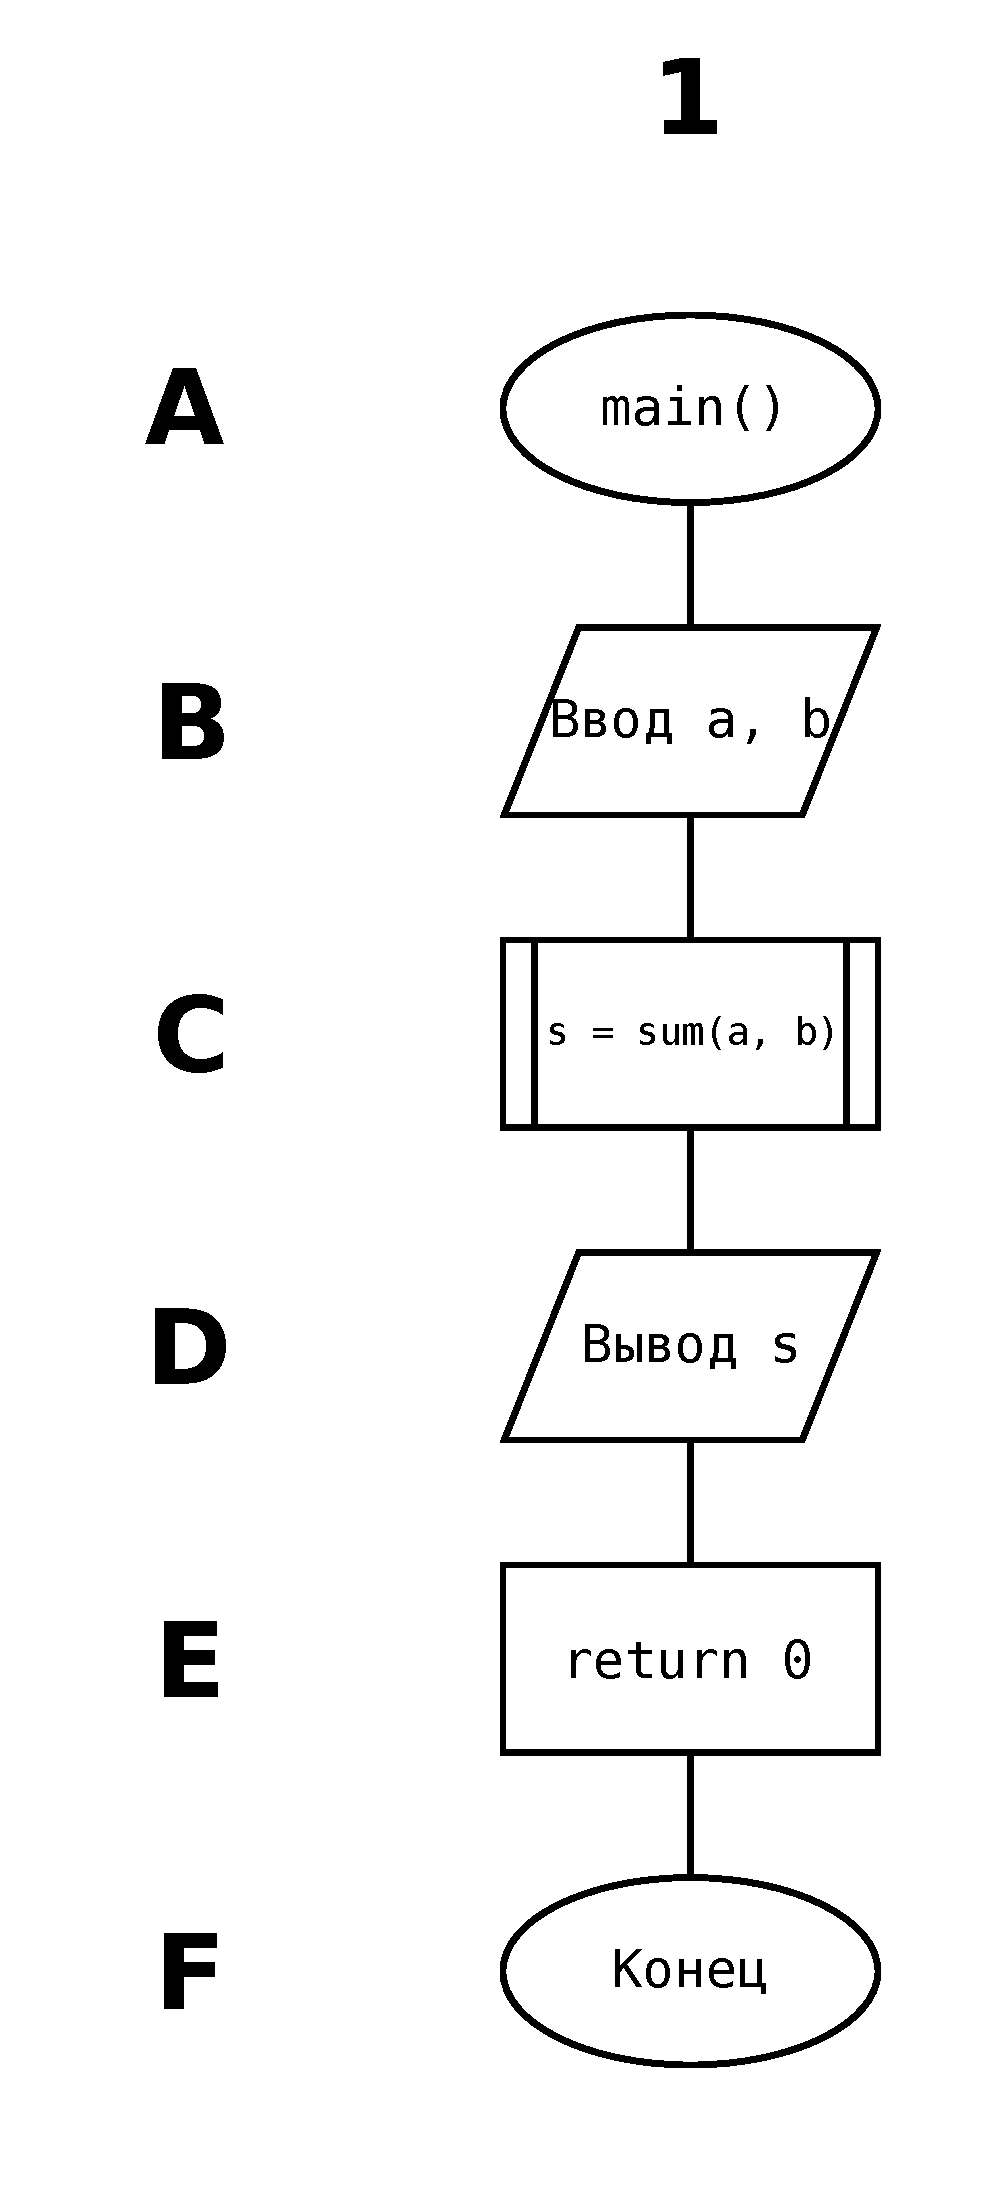
\includegraphics[width=0.4\textwidth]{fc_main}
  \caption{Блок-схема алгоритма работы функции \texttt{main()}}
\end{figure}

\begin{figure}[H]
  \centering
  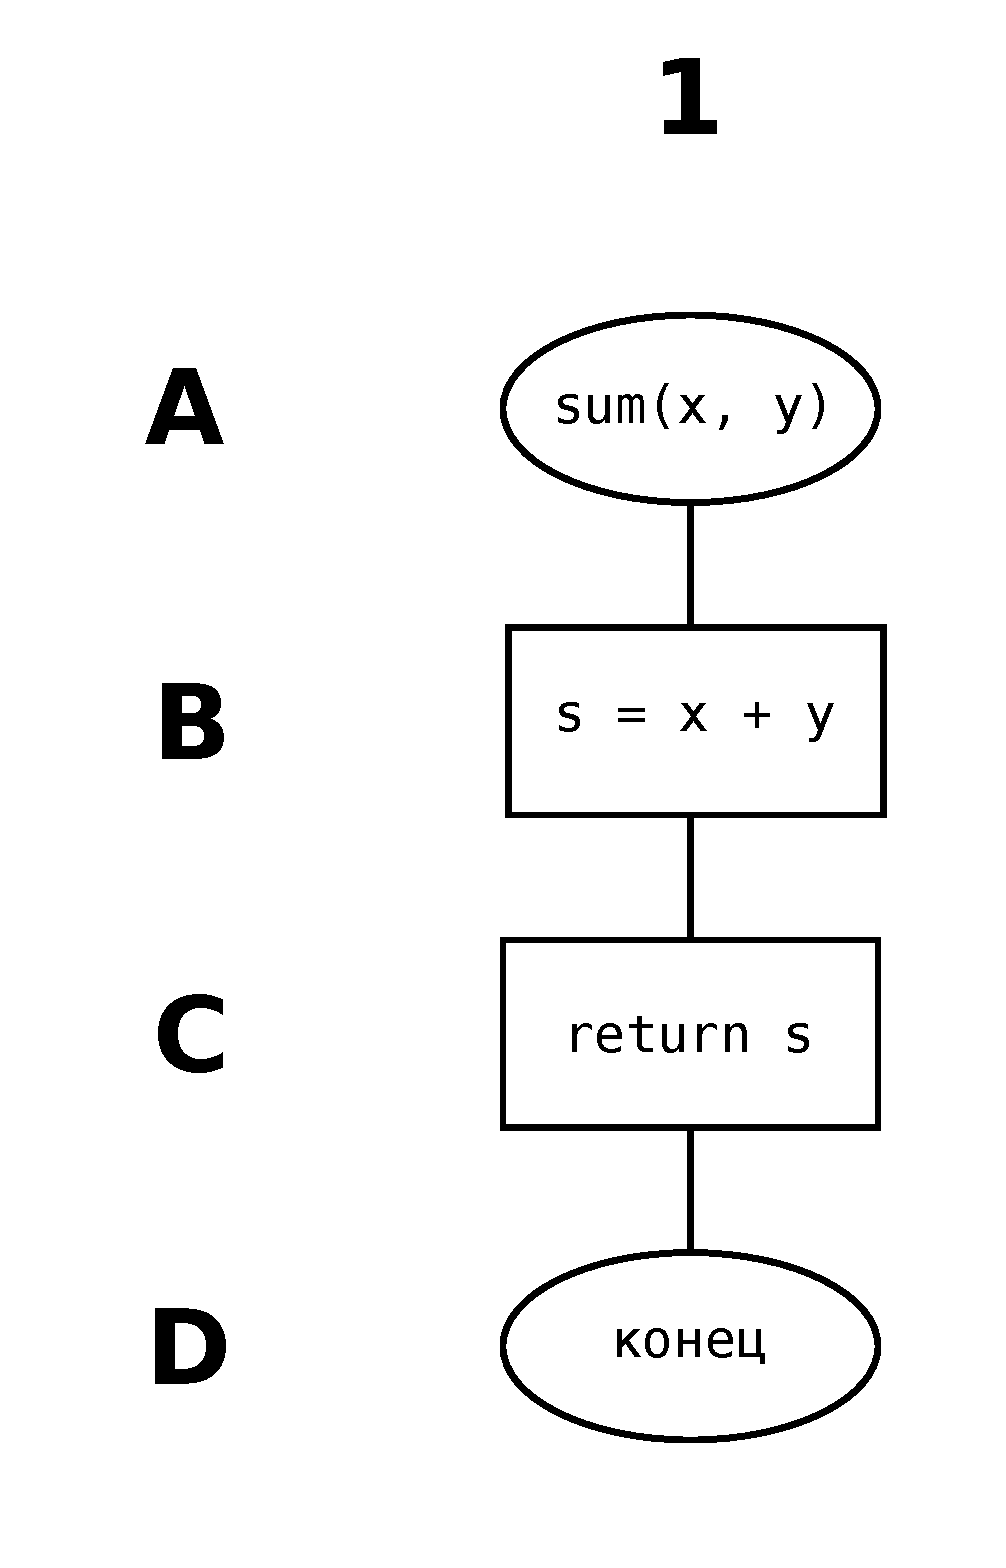
\includegraphics[width=0.4\textwidth]{fc_sum}
  \caption{Блок-схема алгоритма работы функции \texttt{sum()}}
\end{figure}


\section{Исходные коды разработанных программ.}

\begin{lstlisting}
	#include <endian.h>
	#include <stdio.h>
	#include <stdlib.h>
	
	#include "list.h"
	#include "sort.h"
	#include "readline.h"
	
	#define PROMT "----> "
	
	int proccess(List *list)
	{
		if (!list) return -1;
	
		while (list && !list->head) 
		{
			free(list);
			list = readline(PROMT);
			if (!list) return 1;
		} 
	
		while(list->head->symbol == ' ') 
		{
			Node *tmp = list->head;
			list->head = list->head->next;
			free(tmp);
		}
	
		Node *start = list->head, *end = list->head->next;
		Node *prev = start;
	
		while (end)
		{
			if (end->symbol == '\t') end->symbol = ' ';
	
			while (prev->symbol == ' ' && end->symbol == ' ') 
			{
				prev->next = end->next;
				free(end);
				if (end == list->tail) 
				{
					list->tail = prev;
					end = prev;
					break;
				}
				(prev->next != NULL) ? end = prev->next : prev; 
			}
	
			if (end == list->tail)
			{
				sort(start, end, (int (*)(Node *, Node *))compare);
				break;
			}
			if (end->next->symbol == ' ') 
			{
				sort(start, end, (int (*)(Node *, Node *))compare);
				if (end->next->next) 
				{
					start = end->next;
					prev = end;
					end = start;
				}
				else break;
			}
	
			prev = end;
			end = end->next;
		}
		if (list->tail->symbol == ' ')
		{
			Node *ptr = list->head;
			while (ptr->next != list->tail) 
			{
				ptr = ptr->next;
			}
			list->tail = ptr;
			free(list->tail->next);
			list->tail->next = NULL;
		}
		return 0;
	}
	
	int main()
	{
		List *list = NULL;
		while (1)
		{
			list = readline(PROMT);
			if (!list)
			{
				printf("\n");
				break;
			}
			listPrint(list);
			int error = proccess(list);
			if (error == 0) listPrint(list), listDelete(list);
		}
		return 0;
	}
\end{lstlisting}


\section{Описание тестовых примеров}

\begin{table}[H]
  \centering
  \begin{tabular}{|| c | c | c ||}
    \hline
    Значение \texttt{text} & Ожидаемое значение \texttt{t} & Полученное значение \texttt{t} \\
    \hline\hline
    "bca bca" & "abc abc" & "abc abc" \\
    \hline
    "   dcba    cba ba    a    " & "abcd abc ab a" & "abcd abc ab a" \\
    \hline
    "" & "" & "" \\
    \hline
    ctrl + d &  &  \\
    \hline
  \end{tabular}
  \caption{Тестовые примеры}
\end{table}

\section{Скриншоты}

\begin{figure}[H]
    \centering
    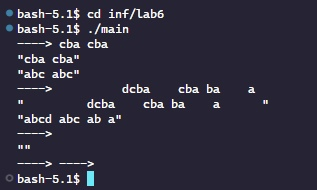
\includegraphics[width=0.9\textwidth]{6proof}
    \caption{Сборка и запуск программы \texttt{main}}
  \end{figure}

\section{Выводы}

В ходе выполнения данной работы на примере программы, выполняющей
ввод и сортировку строки, заданного на физическом уровне в виде списка, были рассмотрены принципы
построения программ на языке C и сортировки строки, заданной на физическом уровне в виде списка:

\begin{enumerate}
    \item Ввод и использование списка.
    \item Организация ввода/вывода списка.
    \item Разработка функций, обрабатывающих список.
    \item Выполнение сортировок над
    строкой, заданной в виде списка.
\end{enumerate}

\end{document}